
\documentclass{article}
\usepackage{ucs}
\usepackage[utf8x]{inputenc}
\usepackage[T1]{fontenc}

\usepackage{graphicx}
\usepackage{tipa}

\usepackage{hyperref}
\usepackage{graphics}


\begin{document}

\title{A constraint grammar for Faroese}
\author{Trond Trosterud \\ 
University of Tromsø \begin{figure}  \scalebox{0.10}[0.10]{
\includegraphics{img/LogoEngelsk}} \end{figure} 
}
\date{}

\maketitle

\begin{abstract}
The present paper presents ongoing work on a finite-state transducer, a Constraint Grammar disambiguator and a dependency grammar for Faroese. In Faroese, the classical Germanic system of case, person and number inflection is upheld, but with somewhat more homonymy than in the closely related Icelandic. Rather than conflating homonym categories, the present morphological transducer gives a fully specified analysis of all morphological distinctions. 
\end{abstract}

\section{Introduction} 

... two words on the parser ...

... presenting this article ...

\subsection{Background}

The transducer is based upon the lemma list of \emph{Føroysk órðabók} (\cite{Poulsen98})\footnote{Thanks to the authors for making lemmalist and inflection codes electronically accessible, Without it this project would of course not have been realisable.}, and upon the grammatical description found in Thráinsson, Petersen, í Lon Jacobsen, Hansen: \textit{Faroese: An overview and reference grammar} 

The Faroese parser uses the computational infrastructure from the Sámi parser project (\textit{giellatekno.uit.no}). It has the same file setup, similar makefiles, etc. There are also benefits in the opposite relation: The Sámi morphophonology testsuite was taken from work on the Faroese \textit{twolc} file. 

The Faroese morphological analyser/generator \textit{Ffst} is a finite-state transducer. It is compiled with Xerox transducer compilers: \textit{twolc} for Morphophonology, and \textit{lexc} for lexicon and morphology (cf. \cite{Beesley03} and \url{http://www.fsmbook.com/}). The disambiguator \textit{Fdis} and dependency grammar \textit{Fdep} are written within the Constraint Grammar framework (see e.g. \cite{Karlsson90}, \cite{Karlsson95}), and uses the 3rd generation compiler \textit{vislcg3} (\cite{Bick00}, \url{http://beta.visl.sdu.dk/cg3.html}).


\section{The morphological analyser}




\subsection{Lexicon}

The analyser uses the same inflectional codes as  \textit{Føroysk orðabók}.  New words annotated with the same codes may thus be added directly to the fst. The analyser has a dynamic compounding component (gen. sg. -> Nouns)

Included in the result is a name guesser. Based upon capital first letter and non-Faroese phonotax the guesser is very reliable: Of the 500 most common guesses all 500 were actually names. 

The name guesser detects words with capital first letter and non-Faroese phonotax. The candidate words must contain at least one vowel. The final letter cannot be a Faroese suffixal sound (\textit{a, i, u, n, m, r, s, t} (to avoid explicit case endings). The putative name is then assigned Nom, Acc and Dat. If there is any other analysis available, the guessed form is automatically discarded. The guesser is very reliable: Of the 500 most common guesses all 500 were actually names. It is also (too) careful: Banning Faroese case suffixes from the guesser avoids analysig case-inflected forms as baseforms, but at the same time it prevents the parser from making many correct guesses. 


\subsection{Morphology and morphophonology}

The morphological part of \textit{Fdis} is built in several layers. For the nominal morphology, the layer structure is as follows:

\begin{enumerate}
\item Part of speech and gender tag, morphophonological flags
\item Case and number morphology
\item Definiteness morphology
\end{enumerate}


\scalebox{0.55}[0.55]{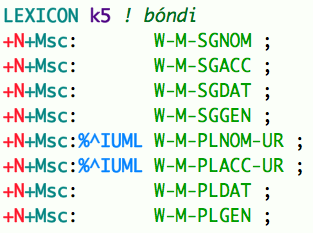
\includegraphics{img/bondi.png}} \\\subsection{Second layer - case and number} 
\scalebox{0.40}[0.40]{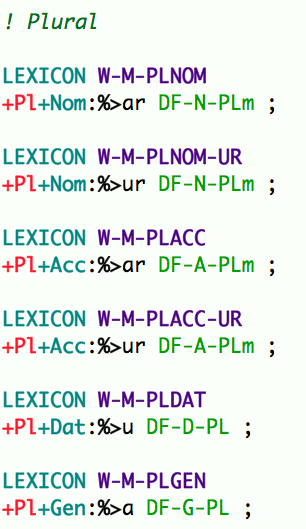
\includegraphics{img/wmplnom.png}} \\\subsection{Third layer - definiteness} 
\scalebox{0.36}[0.36]{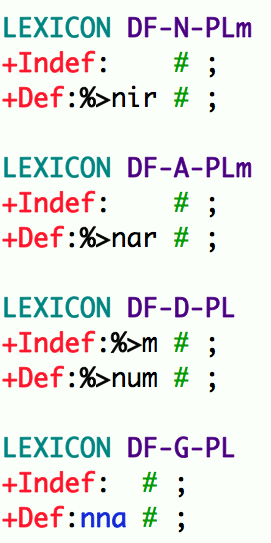
\includegraphics{img/dfnplm.png}} \\\subsection{The resulting upper and lower lexc strings} 


\scalebox{0.40}[0.40]{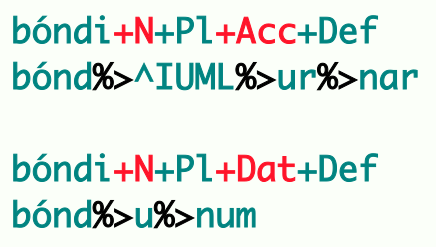
\includegraphics{img/bondi_lexc.png}} \\\subsection{The twolc i-umlaut rule} 
\scalebox{0.45}[0.45]{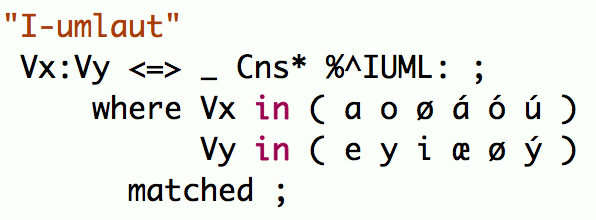
\includegraphics{img/twoliumlaut.png}} \\\subsection{The transducers} 
\scalebox{0.53}[0.53]{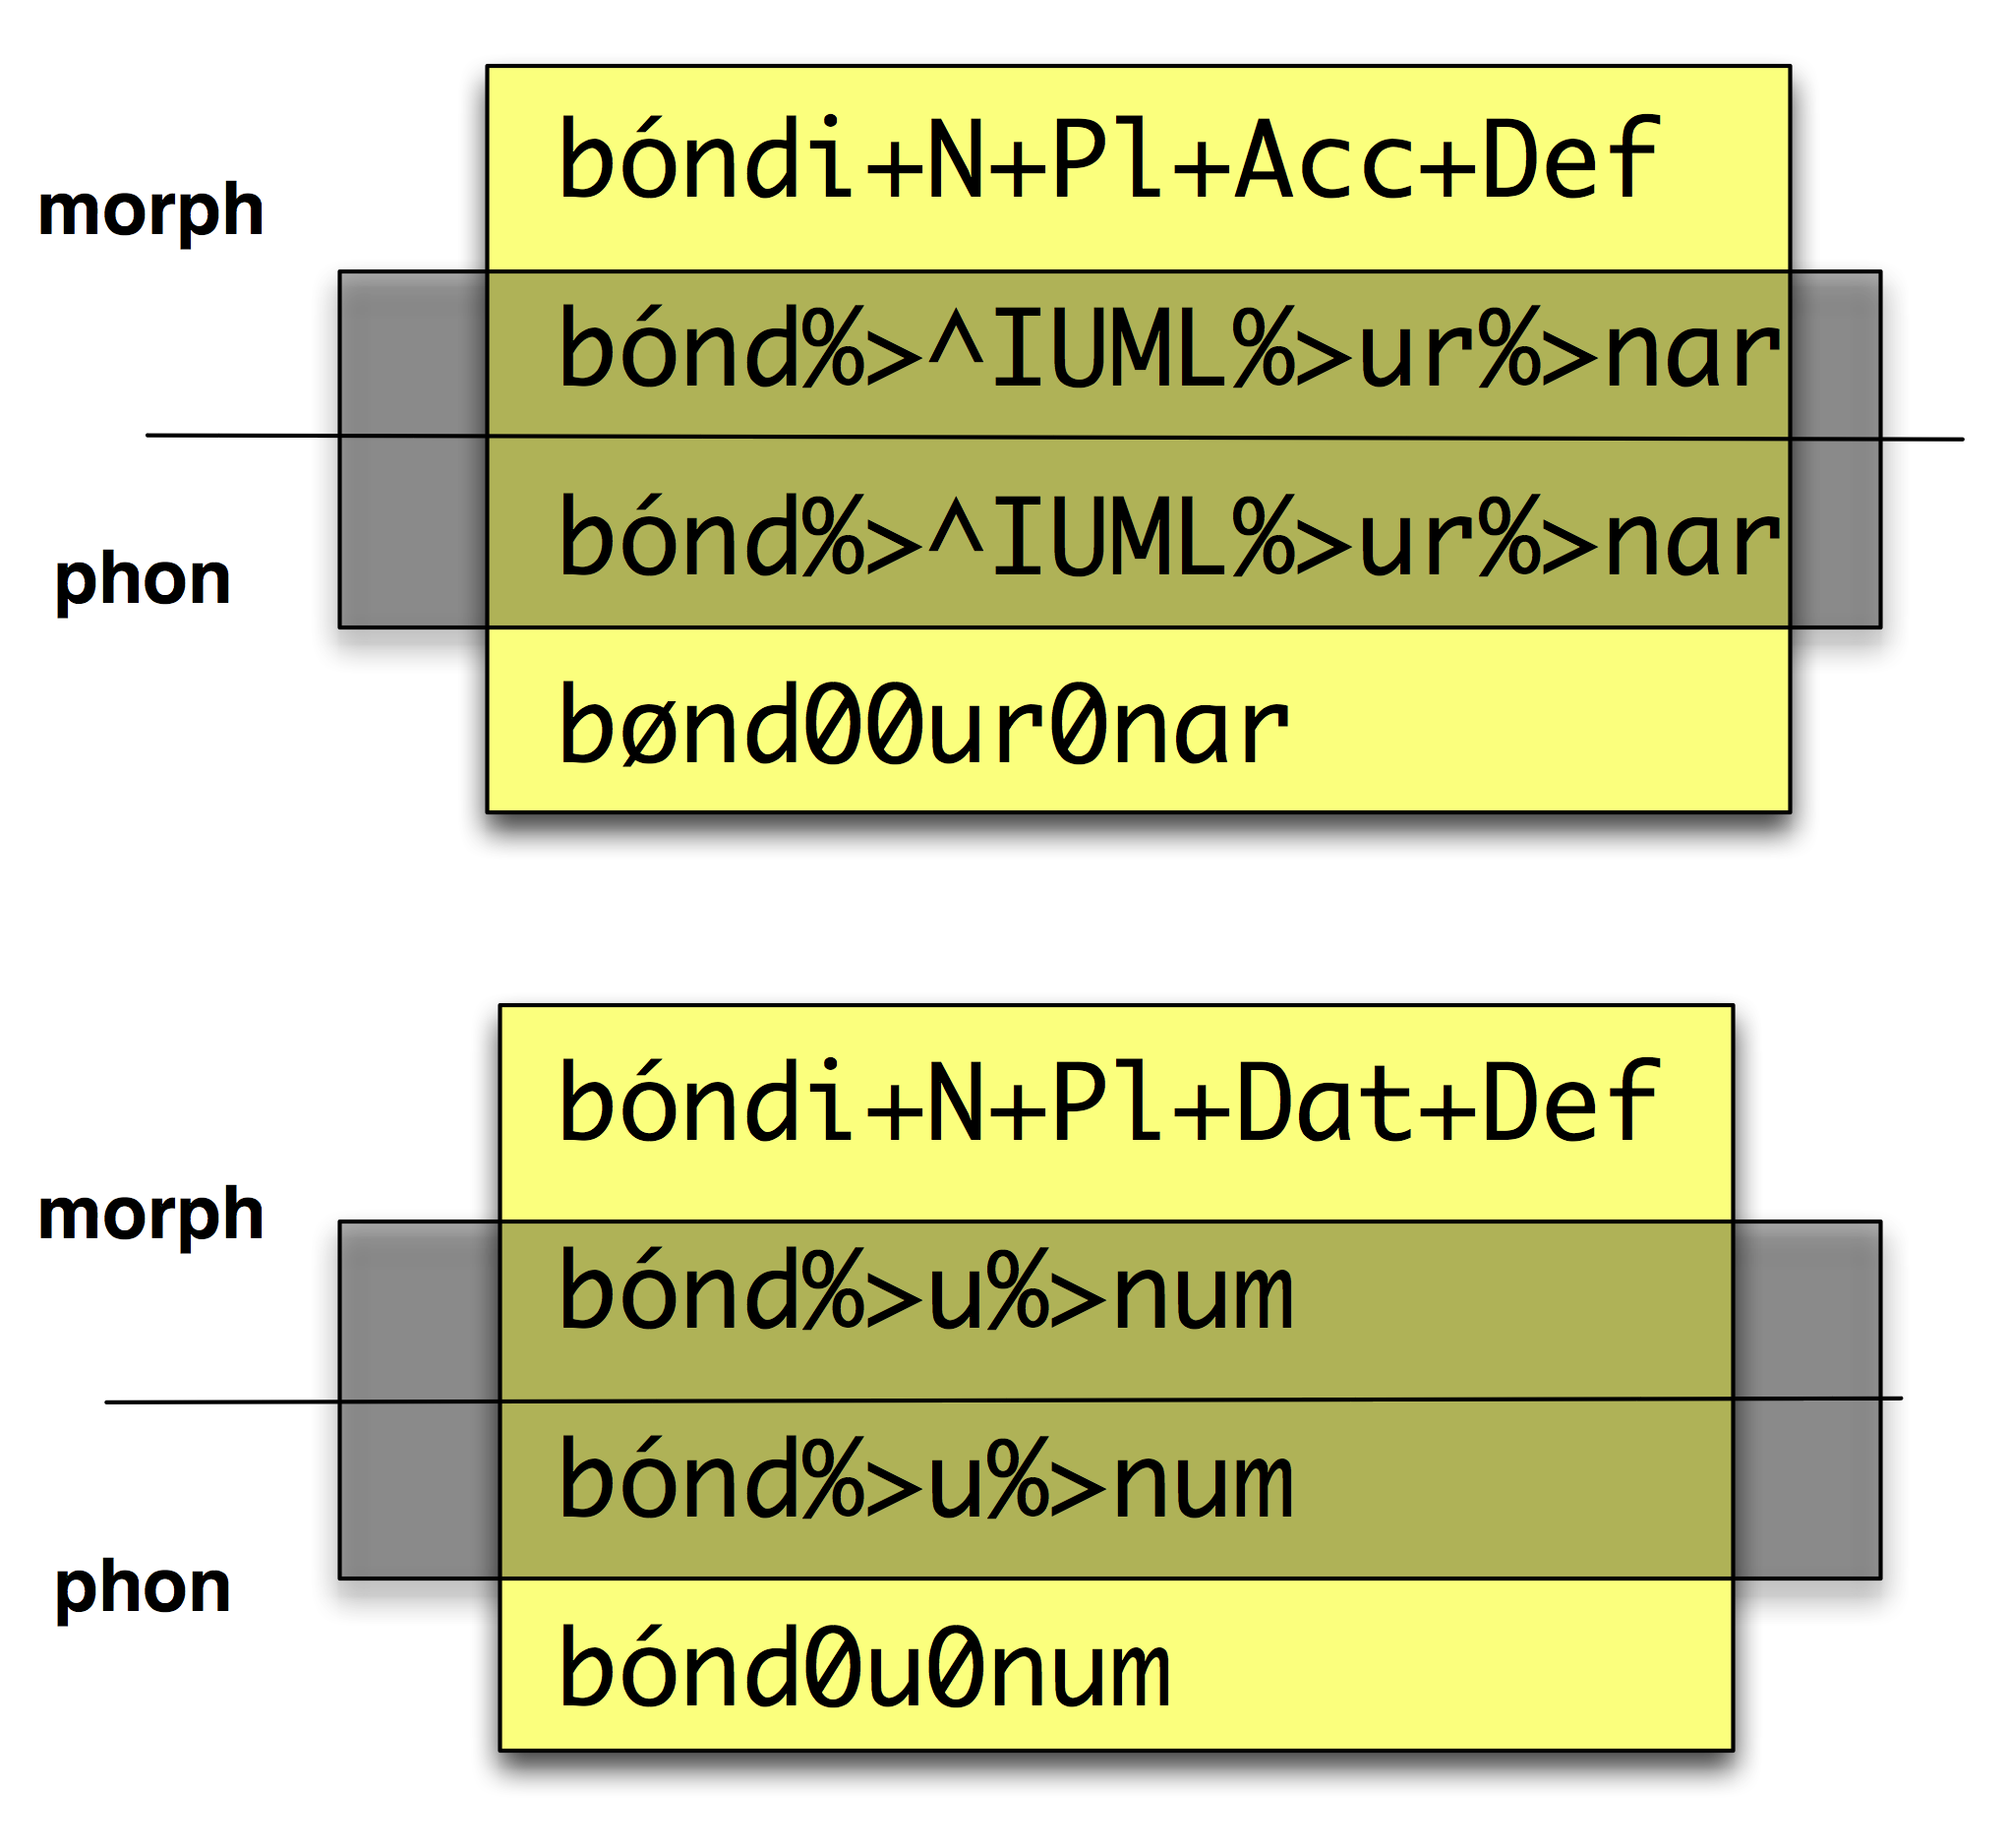
\includegraphics{img/automaton.png}} \\\subsection{The resulting paradigm for bóndi} 
\scalebox{0.33}[0.33]{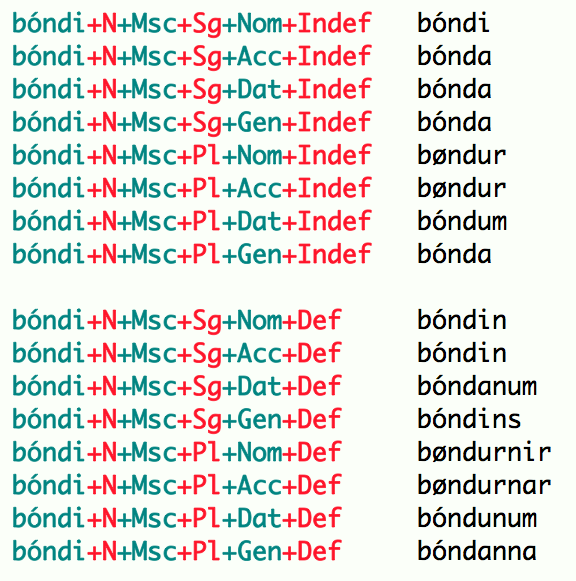
\includegraphics{img/bondiparadigm.png}} \\

\scalebox{0.29}[0.28]{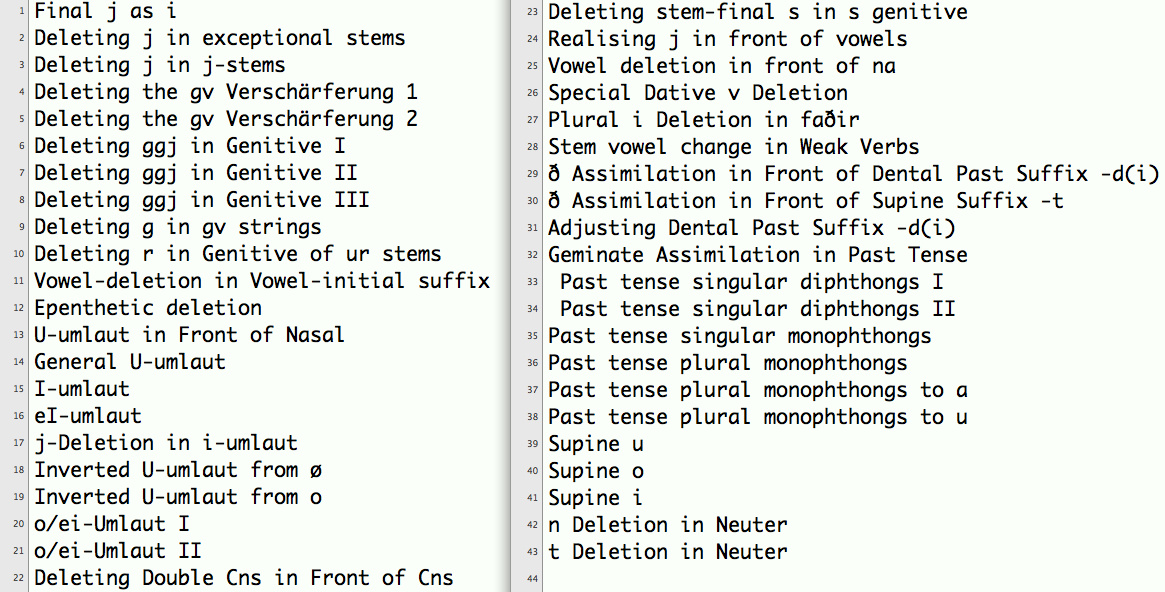
\includegraphics{img/twolrules.png}} \\

\subsection{Status quo for Ffst}


At present (May 2009), the Faroese morphological transducer recognises 93.5 \% of all wordform tokens and 62.8 \% of all wordform types in running text (the discrepancy indicates that Ffst handles common words better than rare ones). 

The results could still be better, but for certain known subgenres (such as the Bible), Ffst gives better results (96.3 \% and 83.3 \%, respectively), results good enough to evaluate the subsequent CG component. Note that even for the known text, Ffst misses approximately 16 \% of the wordform types. The reason for this high number is that certain parts of the transducer are still under construction, especially parts of the irregular verbs, and of comparative and superlative forms of adjectives.

\begin{itemize}
\item The parser recognises 94.3 \% of the wordforms and 63.3  \% of the wordform types in running text
\item The discrepancy indicates that Ffst handles common words better than rare ones
\item{Certain common forms are missing (some strong verbs, irregular adjective forms, comparatives (partly))}
\item{Faroese names are missing (except the most central person names), but many are taken care of by the guesser}
\end{itemize}


The top 84 missing wordforms from an 2.7 m wd corpus

\scalebox{0.33}[0.33]{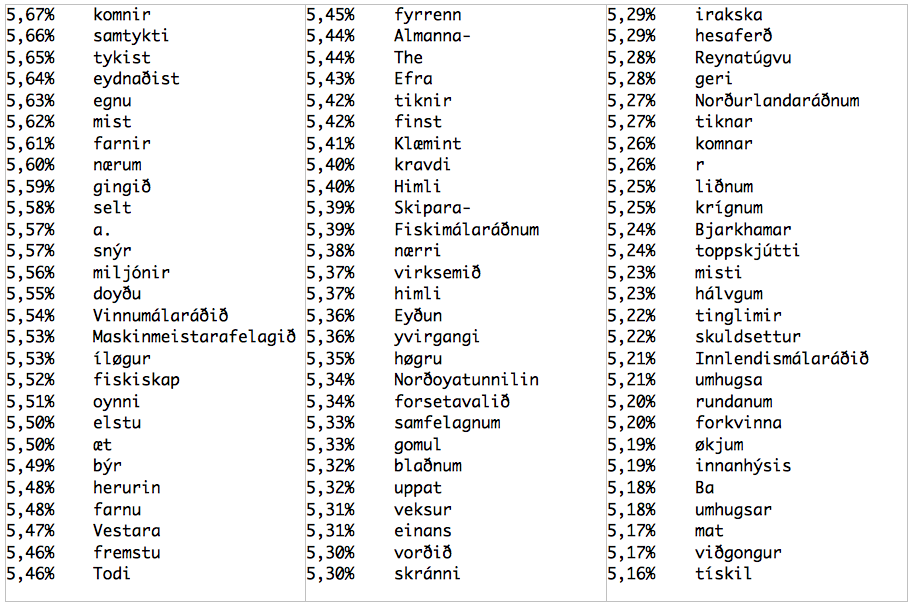
\includegraphics{img/missing.png}} \\


The missing words

\begin{itemize}
\item The 43093 missing words represent 5.67\% of the 2.7 mill corpus. 
\item In order to reduce the number of missing words in running text by 50\%, the top 2117 wordforms of the missing list would have to be added to the analyser. \\ 
\item Important areas for lexicon improvement
\begin{itemize}
\item Adjectival inflection of participles, irregular adjectival forms
\item Some irregular strong verbs and verb forms
\item Faroese names (other than person names)
\item Compounded function words
\item Words missing from FÓ
\item Plain errors
\end{itemize}



\end{itemize}\subsection{The Faroese disambiguator}

The disambiguator (Fdis) consists of

\begin{itemize} 
\item 120 rules for morphological disambiguation, 
\item 49 mapping rules, 
\item 46 rules for GF-disambiguation. 
\end{itemize}

This is a small, but relatively efficient rule set, compared to the disambiguators for some other languages in Table \ref{rulecount}\footnote{telling what and when}.

\begin{table}[htdp]
%\caption{rulecount}
\begin{center}
\begin{tabular}{|l|c|c|c|}
\hline
Parser & Rules & Input ambiguity & disambiguated output \\
\hline
North Sámi	  & 3537 & 2.42 & 1.08 \\
Norsk Bokmål  & 1964 & 2.13 & 1.17 \\
Lule Sámi	  &  832 & 2.18 & 1.21 \\
Faroese		  &  294 & 2.45 & 1.24 \\
Greenlandic	  &  518 & 2.69 & 1.42 \\
\hline
\end{tabular}
\end{center}
\label{Rules and results for som CG parsers}
\end{table}%

\subsection{Tag unification}

The efficiency of the ruleset illustrates the efficiency of an innovation in vislcg3, namely set unification for tags. 

With the set unification operator $\$\$$ it is possible to refer to a set, so that the tag that first satisfies the set must be the same as all subsequent matches of the same set.

\begin{itemize}
\item SET NAGD = Nom Acc Gen Dat ;
\item SELECT \$\$NAGD IF (0 Det)(*1C \$\$NAGD BARRIER NOT-NP);
\end{itemize}



The disambiguator (Fdis) consists of 120 rules for morphological disambiguation, 49 mapping rules, and 46 rules for GF-disambiguation. The dependency grammar (Fdep) consists of 49 rules. With this rule set, Fdis works with an accuracy of 1.14 (an average of 1.14 analyses per word in running text), on an input where the wordforms on average had 3.01 analyses (the results were obtained on a corpus of 100000 words of newstext , previously not used for rule development, disregarding the unknown words, who had no cohorts to disambiguate).

Remarkable here is the low number of disambiguation rules. A standard CG grammar usually has several thousand rules. Partly, the low number of rules in Fdis reflects the intermediate status of the parser, and also its low accuracy (for a CG parser an accuracy of 1.14 is not a good result), but partly it illustrates the efficiency of an innovation in vislcg3, namely set unification for tags. With the set unification operator \$\$ it is possible to refer to a set, so that the tag that first satisfies the set must be the same as all subsequent matches of the same set. Cf. (\ref{NAGD}), where the case of the determiner is selected based upon any unambiguous case form within the same NP.

\begin{example}\label{NAGD}
SELECT \$\$NAGD IF (0 Det)(*1C \$\$NAGD BARRIER NOT-NP);
\end{example}

The bulk of the rules aims at disambiguating case, number and gender within the NP. One clue as to determining the correct case is the choice of preposition, as it is for the human listener. Unfortunately, most Faroese prepositions subcategorise for more than one case. What case to choose if there is a tie is ultimately dependant upon the combination of verb and preposition. At the present stage, Fdis does not specify subcategorisation frames for verbs and verb + preposition combinations, this is an area for future improvement.

When disambiguating running text, certain high-frequent words need special attention, both because they get multiple interpretations in the morphological component, and for their key role in the sentence. A common strategy for such words is to write specific rules just for these words. For Fdis, only approximately 15 such words have received special treatment until now, among them the pronouns \textit{hon, vit} and the ambiguous function words \textit{at, ið, men}. Also this is an area for improvement.

The Faroese verbal paradigm shows much homonymy. Ffst follows the practice of the reference grammars, and specifies 3 persons in the singular (also when the conjugation in question shows homonymy), but only one plural form. Naturally, disambiguating of the verbal forms rests heavily upon the person of the subject. 

Mapping of grammatical functions is done on the basis of morphological cues and word order, and their disambiguation mainly on the basis of word order. The grammatical function tags are directional (the distinction @OBJ> / @<OBJ indicates whether the governing verb is to found to the right or to the left, respectively). This distinction is heavily utilised in the dependency grammar.

The dependency grammar quite reliably delimits NPs, and the governed constituents of P and V. Eventual errors here are due to errors in Fdis. The main obstacles for a good depencency analyses are coordination and relative clauses. Attaching appropriate constituents to the clause mother node is quite a reliable process as long as the rest of the analysis is correct. Unfortunately shortcomings in coordination and relative clause analysis, and especially the low coverage of the Ffst gives too many top nodes (2.3 alleged clausal heads per clause on average, compared to the correct 1 head/clause). Even with these shortcomings, the Fdep is already at this stage a good tool for research on basic dependency relations.


Unfortunately, most Faroese prepositions subcategorise for more than one case.  The choice of case is ultimately dependant upon the combination of verb (or sentence frame) and preposition.  Approach: Select Acc for motion verbs and change of relationship PPs, otherwise go for Dat.

Verb disambiguation is a key area as well}


\subsection{High-frequent ambiguous words}

\begin{itemize}
\item Certain high-frequent words need special attention, 
\begin{itemize}
\item both because they get multiple interpretations in the morphological component, and 
\item for their key role in the sentence.
\end{itemize} 
\item A common strategy for such words is to write specific rules just for these words.  \\ 
\end{itemize} 

For Fdis, only approximately 15 such words have received special treatment until now:

\begin{description}
\item [Pronouns:] \textit{hon, vit, ..}
\item [Subjunctions:] \textit{at, ið, men, ...}
\end{description}
\subsection{Verb homonymy}

\begin{itemize}
\item The Faroese verbal paradigm shows much homonymy. 
\begin{itemize}
\item Ffst specifies 3 persons in the singular (also when the conjugation in question shows homonymy), 
but there is only one plural form (no disambiguation here). 
\end{itemize} 
\end{itemize} 

\subsection{Grammatical functions}

\begin{itemize}
\item Mapping of grammatical functions by
\begin{itemize}
\item morphological cues
\item word order
\end{itemize}
\item and disambiguation of grammatical functions by
\begin{itemize}
\item word order \\ 
\end{itemize}
\item The grammatical function tags are directional 
\begin{itemize}
\item ( @OBJ> / @<OBJ )
\end{itemize}
\item This distinction is heavily utilised in the dependency grammar.
\end{itemize}\section{The dependency grammar}
\subsection{The dependency grammar}

\begin{itemize}
\item The dependency grammar (Fdep) consists of 49 rules. 
\item The dependency grammar quite reliably delimits NPs, and the governed constituents of P and V. 
\begin{itemize}
\item Eventual errors here are due to errors in Fdis. 
\end{itemize}
\item The hard obstacles for a good depencency analyses are long-distance dependencies: 
\begin{itemize}
\item coordination and relative clauses, topicalisation.
\end{itemize}
\end{itemize}

\subsection{The dependency grammar}

\begin{itemize}
\item Shortcomings in coordination and relative clause analysis, and especially the low coverage of the Ffst gives too many top nodes 
\begin{itemize}
\item 2.3 alleged clausal heads (i.e., fragments) per clause on average, compared to the correct 1 head/clause \\ 
\end{itemize}
\item Even with these shortcomings, the Fdep is already at this stage a good tool for research on basic dependency relations.
\end{itemize}\section{Evaluation}
\subsection{Precision and recall}

The parser was tested on a small corpus of 1033 words of unseen text from a new genre (Faroese education planning)

\begin{table}%[htdp]
%\caption{default}
%\begin{center}
\begin{tabular}{|l|r|r|r|r||r|r|r|r|r|}
\hline
Error type	& tp		& fp		& tn		& fn	& prec	 & rec.	& acc.	& F-ms. \\
\hline
Morphology  &  2048  &  369  &  2501  &  101  &  0.85  &  0.95  &  0.91  &  0.90 \\
Syntax  &  1902  &  515  &  2357  &  245  &  0.79  &  0.89  &  0.85  &  0.83 \\
Dependency  &  724  &  316  &  0  &  0  &  0.7  &  1  &  0.7  &  0.82			  \\
\hline
\end{tabular}
%\end{center}
%\label{default}
\end{table}%

\\ 
-> Fdis is work in progress 
\subsection{Some sentences 1} 
\scalebox{0.40}[0.40]{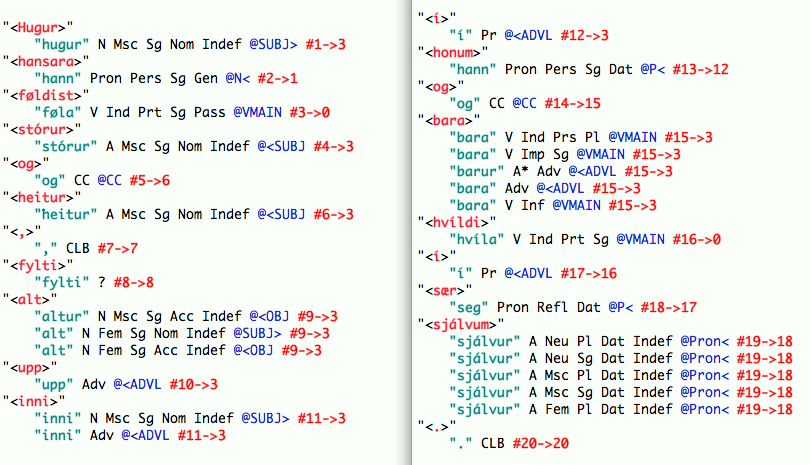
\includegraphics{img/hugur.png}} \\\subsection{Some sentences 2} 
\scalebox{0.50}[0.50]{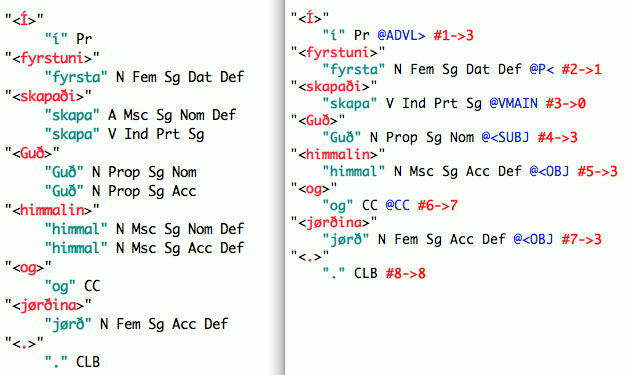
\includegraphics{img/fyrstuni.png}} \\\subsection{Some sentences 3} 
\scalebox{0.30}[0.30]{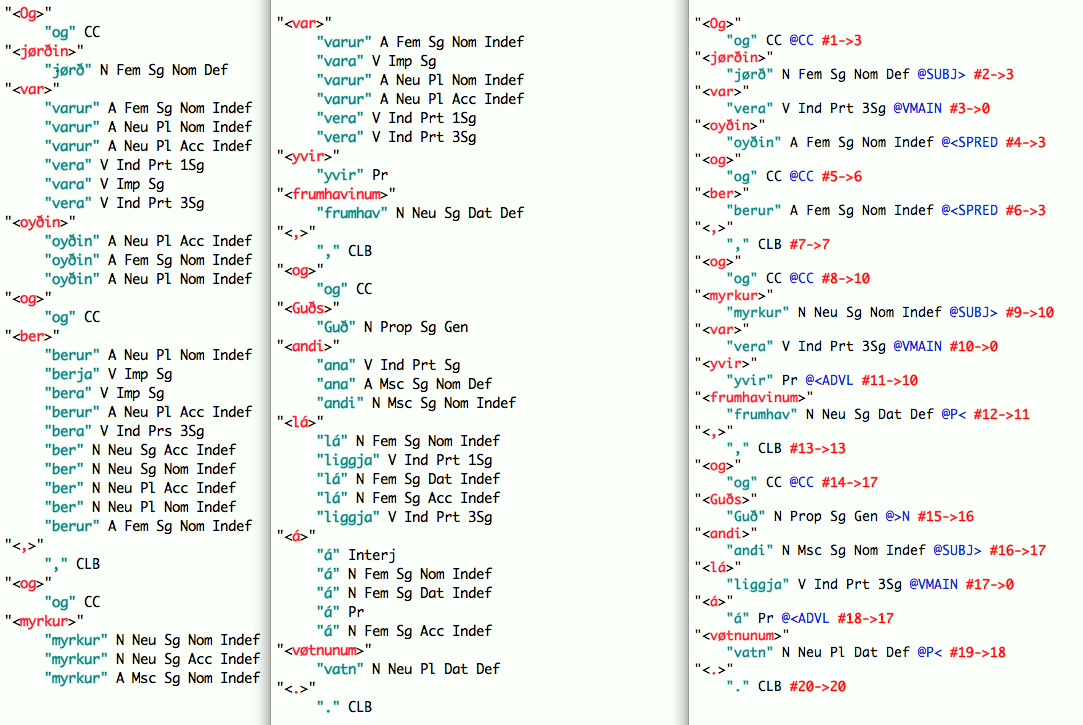
\includegraphics{img/frumhavinum.png}} \\



\section{Processing speed}

When it comes to processing speed, it seems that the bottleneck in the system is the disambiguator. Even though it is much smaller than most CG grammars, it performs clearly worse than all the other parts of the pipeline. The reason for this might be the extensive use of set unification.


\begin{table}[htdp]
\caption{Processing speed, measured on 100000 words of running text, on a 2,4 GHz laptop}
\begin{center}
\begin{tabular}{|l|l|r|}
\hline
Process & Program & Words/sec \\
\hline
Preprocessing & perl &10446 \\
Morphological lookup & fst & 42992 \\
Postprocessing & perl & 13017 \\
Disambiguation & vislcg3 & 2042 \\
Dependency & vislcg3 & 18814 \\
\hline
\end{tabular}
\end{center}
\label{time}
\end{table}%




\subsection{Conclusion}

The Faroese grammatical analyser presented here is still in the making. It still shows that with a modest number of CG rules, one may achive results good enough for several languaguage processing tasks. Future improvements of the analyser will concentrate upon key parts of the Ffst, upon disambiguation of complex syntactic patterns, and upon the dependency analysis of coordination and relative clauses.


\bibliography{$GTPRIV/plan/art/bib/lgtech}

\bibliographystyle{plainnat}

\end{document}
